\section{Experiments} 
\label{sec-experiments}	
 
 	In \cite{lamas2015}, Vilches and Demeulemeester 
 	compare their method (CCP) with 
 	that by Van de Vonder et al. (STC) \cite{van2008}.
 	To the best of our knowledge, STC and CCP constitute the state-of-art as far as
 	trading expected makespan for instability in stochastic project scheduling is concerned.
 	In this section we extend this comparison by using the same experimental set-up
 	and including results for our LP-based heuristic (Section~\ref{sec-lp}) and 
 	the MILP-based heuristic (Section~\ref{sec-milp-heuristic}).
 	As the results show, our approaches compare favorably with STC and CCP.  

  	The set-up used in \cite{lamas2015} was based 
  	on the \texttt{J30} deterministic RCPSP bench-set of the well-known PSPLIB \cite{kolisch1997psplib},
 	which comprises 480 deterministic RCPSP instances, each with $n=30$ activities.
 	Based on this bench-set, three stochastic RCPSP bench-sets were derived, 
 	namely \texttt{J30-low}, \texttt{J30-med}, and \texttt{J30-high},
  	corresponding to conditions of low, medium, and high project uncertainty,
 	with activity durations following a discretized beta distribution.
 	Specifically, each activity $i$ with duration $d_i$ in the deterministic RCPCP instance
 	now has stochastic duration $D_i = [X_i d_i 0.5 (l + h)]$ with $\mathbb{E}[D_i] \simeq d_i$ where
 	\begin{itemize}
 		\item $X_i$ follows a beta distribution with shape parameters $\alpha=2, \beta=5$;
 		\item $l = 0.75$ and $h = 1.625$ in the low variability bench-set;
 		\item $l = 0.5$ and $h = 2.25$ in the medium variability bench-set;
 		\item $l = 0.25$ and $h = 2.875$ in the high variability bench-set;
 		\item operator $[\cdot]$ represents rounding to the closest integer.
 	\end{itemize}

 	Each of the evaluated methods (including STC and CCP) has a certain "tradeoff parameter"
 	which determines whether more emphasis is put on minimizing
 	expected makespan or minimizing expected instability.
 	For our LP-based and MILP-based heuristic this tradeoff parameter 
 	is the weight $\alpha$ in expression (\ref{eq-psrcpsp-obj}).  
 	CCP and STC have corresponding parameters with a similar effect.
 	By varying the choice of the corresponding tradeoff parameter(s),
 	a set of tradeoff data-points is obtained for each method, on each of the three bench-sets.
  
 	\begin{figure} 
 		\centering   
   		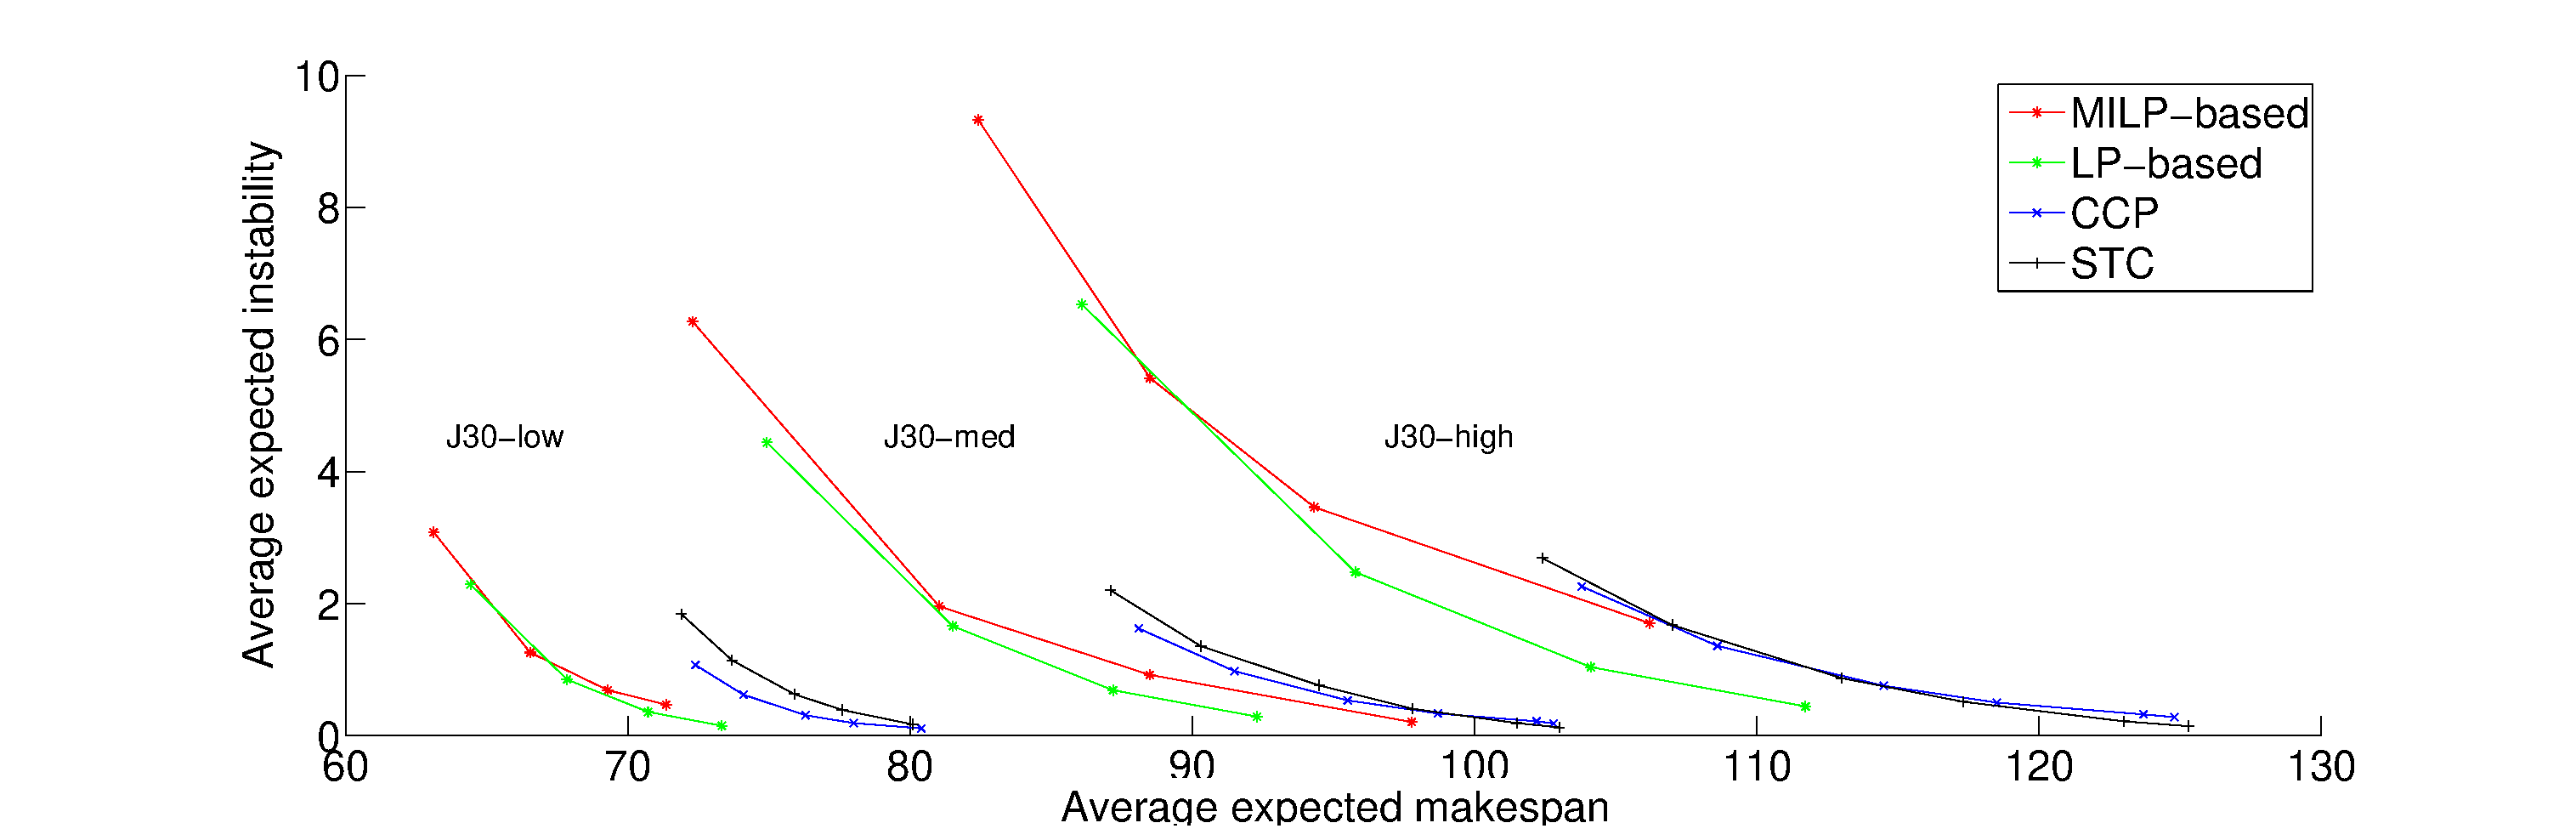
\includegraphics[width=1.0\textwidth]{chapter/mista-stability/figure1.eps}
 		\caption{Trading expected makespan for stability.}
 		\label{fig-experiments-1}
 	\end{figure}
 	
  	\begin{figure} 
 		\centering  
   		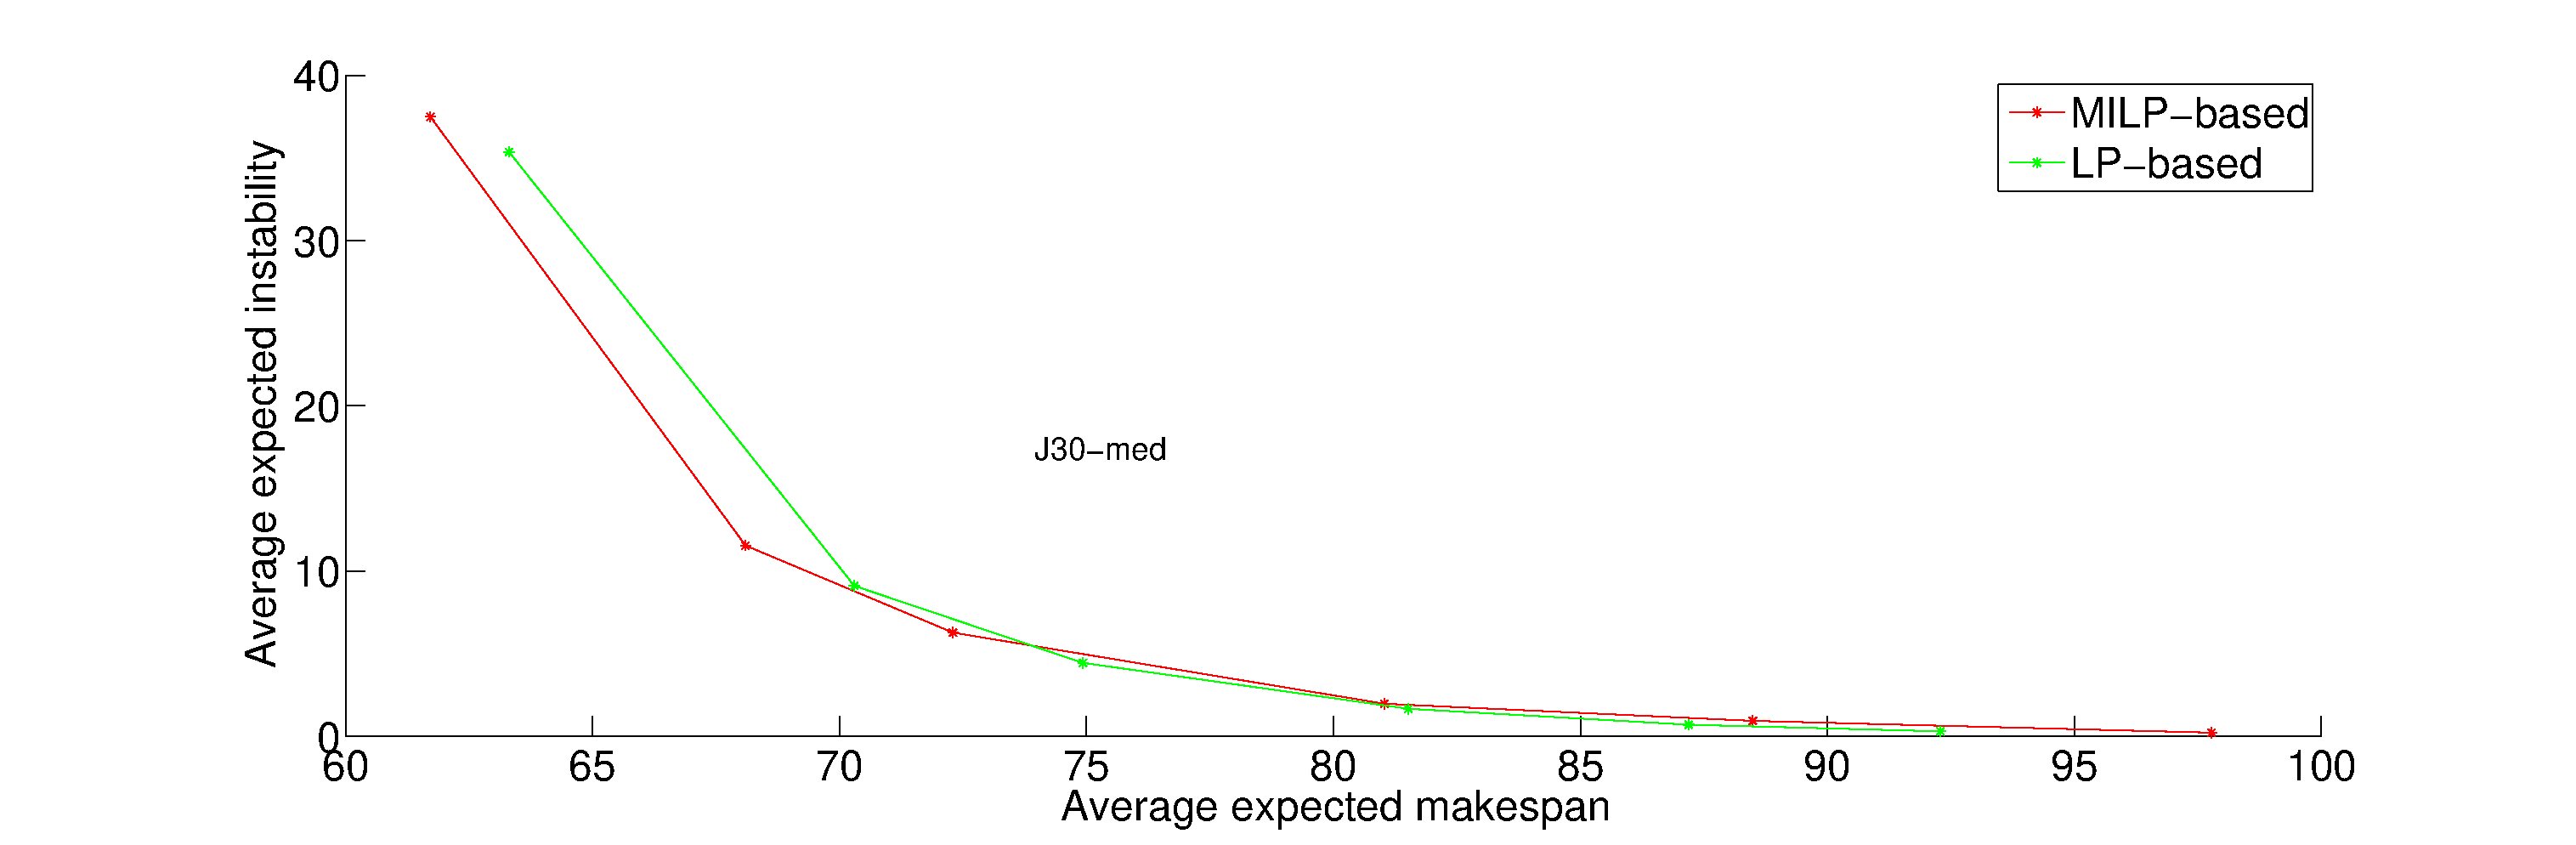
\includegraphics[width=1.0\textwidth]{chapter/mista-stability/figure2.eps}
 		\caption{Trading expected makespan for stability for higher $\alpha$.}
 		\label{fig-experiments-2}
 	\end{figure}
 	
 	In Figure~\ref{fig-experiments-1},
 	the data-points for each method are displayed as a tradeoff curve, 
 	on each of the three bench-sets, resulting in three "clusters" of tradeoff curves.
 	A tradeoff curve captures the average performance of the method on that bench-set.
 	Specifically, each data-point is two-dimensional and records the average expected makespan and average 
 	expected instability for a certain choice of the tradeoff parameter(s),
 	where the average is taken over all 480 instances of the bench-set.
  	Data-points for CCP and STC are borrowed
 	from the work of Vilches and Demeulemeester \cite{lamas2015}.	
  	Data-points for our heuristics are obtained by setting $\alpha=0.05$, $0.1$, $0.2$, and $0.4$.
 	Higher alpha values correspond to data-points closer to the upper left corner,
 	with higher instability and lower makespan.	
 	
 	Figure~\ref{fig-experiments-2} focuses on the medium variability case for higher $\alpha$ values,
 	including additional data-points for $\alpha=0.6$ and $\alpha=0.9$.
 	This allows us to compare the MILP-based and LP-based heuristics when
 	more emphasis is put on minimizing expected makespan.
 	
 	The expected makespan and expected instability of the solution
 	provided by each of the methods on a particular instance
 	is computed with a sample $\Gamma^{large} \subset \mathbb{R}^n$ 
 	comprising $|\Gamma^{large}| = 10^3$ realization of durations vector $\xD$.
 	Note that the data-points of Vilches and Demeulemeester were computed with a different sample of size $10^3$.
 	We assume that $10^3$ is a sufficiently large sample size to facilitate comparability with our results.
 	
 	\paragraph{Configuration of heuristics.}
 	The sample $\Gamma^{milp}$ used by our MILP-based heuristic during optimization
 	(see line 6 of Algorithm~\ref{alg-milp-heuristic}) is of size $|\Gamma^{milp}| = 30$.
 	Our MILP-based heuristic is configured to perform three (3) iterations and
 	the number of highly critical arcs removed in each iteration 
 	(see line 5 of Algorithm~\ref{alg-milp-heuristic}) is $|\mathcal{H}| = 20$.
 	Note that the criticality of the arcs is computed based on sample $\Gamma^{large}$
 	(this is done efficiently, in time quadratic in $n$ and linear in $|\Gamma^{large}|$).
  	The solver we use is \textsc{CPLEX} version 12.6.
  	Furthermore, we set a time-limit for the solver to 50 seconds
  	(since each iteration starts from a feasible solution, 
  	the solver will always return with a solution within the time-limit).
  	The polynomial-time complexity of our LP-based heuristic (no binary variables in the model)
  	allows us to use a large sample during optimization.
  	In fact, we use sample $\Gamma^{large}$.
  	To find a deterministic schedule (as required in step 1 of this LP-based heuristic)
  	we used a priority rule procedure recently proposed in \cite{de2014novel}.
  	Vilches and Demeulemeester use a sample of size $10^2$ during optimization, for both STC and CCP.
  	Furthermore, they limit the time spent in solving their 
  	CCP model on an instance to a maximum of 10 seconds. 
 
   	
  	\paragraph{Observations.}
  	Figure~\ref{fig-experiments-1} suggests that
   	regardless of the mode of variability (low, medium, or high),
  	when the purpose is to achieve near-zero instability,
  	the LP-based heuristic yields the best results.
  	This can be attributed to the efficiency of solving a LP model,
  	which enables us to use a large sample (of size $10^3$ in this case) during optimization.
  	
  	Figure~\ref{fig-experiments-2} suggests that
  	even though the sample used during optimization is much smaller
  	for the MILP-based heuristic (of size $30$),
  	it is more effective than the LP-based heuristic for higher $\alpha$ values
  	(i.e. when minimizing instability is  more important than minimizing makespan).
  	Both the LP-based and the MILP-based heuristics start from the same es-policy
  	(see step 1 in section~\ref{sec-lp} and line 2 of Algorithm~\ref{alg-milp-heuristic}, respectively).
  	However, the MILP-based heuristic restructures the policy and this enables
  	it to perform better at minimizing expected makespan.
  	
  	Restructuring the policy comes at the cost of efficiency.
   	With three iterations allowed per instance,
  	this yields an average of 50 seconds per instance for the MILP-based heuristic.
  	The LP-based heuristic is considerably more efficient, with an average of 1.5 seconds per instance.
  	Vilches and Demeulemeester report that STC spends on average 0.2 seconds per instance,
  	while their CCP approach spends on average 10 seconds per instance. 
 	
